\documentclass[11pt,a4paper,english,oneside]{book}

%----------------------------------------------------------------------------------------
% THESIS SETTINGS - ADAPT
%----------------------------------------------------------------------------------------
% Depending on your program, (un)comment the following lines

% Are you in the Quant finance program?
\newif\ifQF % default behaviour is false, so NOT in QF - always leave uncommented!
% \QFtrue % Uncomment if you are in the QF program, if not leave it out

% Pick One option
\newcommand{\thesis}{Bachelor}
% \newcommand{\thesis}{Master}


% ==========================================================================================
% PREAMBLE
% ==========================================================================================
%----------------------------------------------------------------------------------------
% GENERAL  - PACKAGES
%----------------------------------------------------------------------------------------
% GENERAL
\usepackage{etex}
\usepackage[utf8]{inputenc}

% Mathematical packages
\usepackage{amsmath}
\usepackage{amsfonts}
\usepackage{amssymb}
\usepackage{mathtools}
\usepackage{breqn}

% LAYOUT/PAGE/TEXT FORMATTING
\usepackage[left=1in, right=1in]{geometry}
\usepackage{setspace}
\usepackage{fancyhdr}
\usepackage[hang,bottom,stable,multiple]{footmisc}
\usepackage{dsfont}

\usepackage[svgnames]{xcolor}
\definecolor{MyColor1}{rgb}{0.2,0.4,0.6}

% FLOATS
\usepackage{booktabs}
\usepackage{multirow}
\usepackage{colortbl}
\usepackage{array}
\usepackage{hhline}
\usepackage{rotating}
\usepackage{tabularx}
\usepackage{float}
\usepackage{graphicx}
\usepackage[margin=10pt, font=small, labelfont=bf, labelsep=endash]{caption}

% OTHER ENVIRONMENTS
\usepackage{textcomp}
\usepackage{amsthm}
\usepackage{thmtools}
\usepackage{appendix}
\usepackage{etoolbox}
\makeatletter
\patchcmd{\@chap@pppage}{\thispagestyle{plain}}{\thispagestyle{empty}}{}{}
\makeatother

\usepackage{listings}

% VARIA
\usepackage{epstopdf}
\usepackage{lipsum}
\usepackage{datetime}
\usepackage{chngcntr}
\usepackage{xparse}
\usepackage{arydshln}

% BIBLIOGRAPHY - BIBLATEX
\usepackage[
backend=biber,
style=apa,
bibstyle=authoryear,
citestyle=authoryear,
maxcitenames=2,
maxbibnames=99
]{biblatex}

\setlength\bibitemsep{1\itemsep}
\addbibresource{references.bib}

\usepackage{hyperref}
\hypersetup{
     colorlinks=false,
     linkcolor=blue,
     citecolor=blue,
     filecolor=magenta,
     urlcolor=blue
}

\usepackage[nameinlink,capitalize]{cleveref}

%----------------------------------------------------------------------------------------
% GENERAL  - SETUP
%----------------------------------------------------------------------------------------
\setlength{\textwidth}{6.6in}
\setlength{\textheight}{8.8in}
\setlength{\topmargin}{-0.1in}
\setlength{\oddsidemargin}{0in}
\setlength{\parskip}{1mm}

\setlength{\parindent}{0cm}

\counterwithout{footnote}{chapter}
\numberwithin{equation}{chapter}

\allowdisplaybreaks[1]

%----------------------------------------------------------------------------------------
% CUSTOM COMMANDS/ENVIRONMENTS
%----------------------------------------------------------------------------------------
\makeatletter
  \newcommand{\ud}{\mathrm{d}}
\makeatother

\declaretheorem[style=definition,qed=\(\blacktriangleleft\), numberwithin=chapter]{remark}
\declaretheorem[style=definition,qed=\(\triangle\),numberwithin=chapter]{definition}
\newtheorem{ass}{Assumption}[chapter]
\newtheorem{prop}{Proposition}[chapter]
\newtheorem{lemma}{Lemma}[chapter]
\declaretheorem[style=definition,qed=\(\perp\),numberwithin=chapter]{example}
\newtheorem{theorem}{Theorem}[chapter]
\newtheorem{coroll}{Corollary}[chapter]

%----------------------------------------------------------------------------------------
% TITLE PAGE
%----------------------------------------------------------------------------------------
\newcommand*{\uzhlogo}{
\includegraphics{../thesis_template/Graphics/uzh_logo_e_pos.pdf}}

\newcommand*{\titleGP}{\begingroup
\centering
\vspace*{\baselineskip}
\ifQF
\uzhlogo\\[2\baselineskip]
\else
\uzhlogo\\[2\baselineskip]
\fi

\rule{\textwidth}{1.6pt}\vspace*{-\baselineskip}\vspace*{2pt}
\rule{\textwidth}{0.4pt}\\[\baselineskip]

{\LARGE Understanding Data Mixture Effects in Financial Language Model Pretraining}\\[0.3\baselineskip]
{\large A Study of Domain-Specific and High-Quality General Corpora}\\[0.2\baselineskip]

\rule{\textwidth}{0.4pt}\vspace*{-\baselineskip}\vspace{3.2pt}
\rule{\textwidth}{1.6pt}\\[2\baselineskip]
\scshape

\thesis's Thesis\\[2\baselineskip]

\ifQF
Submitted in partial fulfillment of the requirements for the degree of Master of Science in Quantitative Finance \par
\else
Submitted in partial fulfillment of the requirements for the degree of \thesis\ of Arts in Economics and Business Administration \par
\fi

\vspace*{2\baselineskip}

Student\\
{\Large Guanlan Liu \\ [5pt]
}
19-768-837\\[5pt]
guanlan.liu@uzh.ch \\

\vspace*{2\baselineskip}

Supervisor\\
{\Large Prof.\ Dr.\ Markus Leippold\\[5pt]
\small Professor of Financial Engineering\\[5pt]
\small Department of Finance\\[5pt]
University of Zurich\par}
\vspace*{2\baselineskip}

% Assistant\\
{\Large Min Yang\\[5pt]
}
min.yang2@uzh.ch \par

\vfill

{\scshape Date of Submission: [ Date ]} \\[0.3\baselineskip]

\endgroup}

%----------------------------------------------------------------------------------------
% HEADER/FOOTER
%----------------------------------------------------------------------------------------
\fancypagestyle{firststyle}{%
  \fancyhf{}%
  \renewcommand{\headrulewidth}{0pt}
  \fancyfoot[C]{\thepage}
}

\pagestyle{fancy}
\fancyhead[R]{\thepage}
\fancyhead[L]{\rightmark}
\fancyfoot[L]{Guanlan Liu}
\fancyfoot[C]{}
\fancyfoot[R]{Data Mixture Effects in Financial LM Pretraining}
\setlength{\headheight}{13.6pt}

%----------------------------------------------------------------------------------------
% SIGNATURE SETUP
%----------------------------------------------------------------------------------------
\NewDocumentCommand\dotbox{o O{.5\linewidth} m O{3ex} O{\linewidth}}
{
  \begin{minipage}{7cm}
    \makebox[7cm][l]{\,.\dotfill}
    \\
    \makebox[7cm][l]{\,#3}
  \end{minipage}
}
 % CHECK OUT the preamble.tex file and adapt the necessary parts (use CTRL+f and look for "ADAPT"))

\begin{document}

%----------------------------------------------------------------------------------------
% TITLE PAGE
%----------------------------------------------------------------------------------------
\thispagestyle{empty}
\titleGP\

\newpage

\doublespacing\
\setcounter{page}{1}
\pagenumbering{Roman}

%----------------------------------------------------------------------------------------
% TASK ASSIGNMENT
%----------------------------------------------------------------------------------------
\section*{Task Assignment}
\thispagestyle{firststyle}
\newpage

%----------------------------------------------------------------------------------------
% EXECUTIVE SUMMARY
%----------------------------------------------------------------------------------------
\section*{Executive Summary}
\thispagestyle{firststyle}

%----------------------------------------------------------------------------------------
% 
%----------------------------------------------------------------------------------------
\tableofcontents
\listoffigures
\listoftables

\newpage
\pagenumbering{arabic}


%----------------------------------------------------------------------------------------
% MAIN CHAPTERS
%----------------------------------------------------------------------------------------


%--------------------
% CHAPTER 1
%--------------------


\chapter{[ Chapter Title ]}

\section{[ Section Title ]}

[\dots] Between sections and subsections, you may want to add at least three or four sentences (or more), instead of leaving it blank.

\subsection{[ Subsection Title ]}

The same principle obviously holds for subsequent levels.

\section{\LaTeX\ Basics}

[\dots] In the next subsections, there is the basic information you will need to know and/or is useful to get started with your thesis in \LaTeX. All the packages that are mentioned are already included in the `preamble.tex' file, so you are all set to go to use the presented commands. First, make sure to choose the correct setting on top of this tex file w.r.g. to your program and level (bachelor/master). These settings will automatically lead to the correct title page for your \thesis\ thesis. Next, adapt all the necessary parts (e.g. Author, title, running title, Bachelor/Master, \ldots) in the preamble file.

\subsection{Useful sources}

\begin{itemize} % (see Basics.lists section)
    \item TeX distribution: \href{https://miktex.org/}{MiKTeX} % example for including url's (hyperref and url package)
    \item Editor: \href{https://code.visualstudio.com/}{VSCode}, \href{https://www.xm1math.net/texmaker/}{TeXMaker}, \href{https://www.overleaf.com/}{OverLeaf} (online)
    \item Other resources \href{https://en.wikibooks.org/wiki/LaTeX}{wikibooks}, \href{https://tex.stackexchange.com/}{stackexchange} and \href{http://www.tug.org/interest.html#free}{other}
\end{itemize}

\subsection{Plain text}

You can write simple text in \textbf{bold},  \textit{Italic}, \underline{underlined} or \emph{emphasized}. In different font sizes from {\tiny tiny} to {\Huge Huge}. Also in different colors {\color{Red} red text}, {\color{Green} green text},  {\color{MyColor1} own defined color} \ldots. Obviously, you can also mix things up {\color{Green} \Large \textbf{\textit{test}}}

Be careful with special characters like  \%, \}, \{, \& and \(\backslash\). Indentation is `fixed' with  the  package \emph{setspace}.\footnote{Also for footnotes, thanks to \emph{footmisc}\label{ft:randomfootnote}}. Do not use the simple quotation marks "quote", instead use ``quote''.

\subsection{Lists}
There are different types of so-called list environments: Unordered, Ordered and Description. They can be nested, up to a depth of 4:

\begin{description}
    \item[Description] This type of list (description)
    \item[Unordered] Simple bullet points (itemize)
    \begin{itemize}
        \item Item 1
        \item Item 2
        \item \ldots
    \end{itemize} 
    \item[Ordered] List with order in bullet points (enumerate)
    \begin{enumerate}
        \item Item 1
        \item Item 2
        \item \ldots
    \end{enumerate} 
\end{description}


\subsection{Math and Equations}
You have in-line math environments, for example good for the use of a subscript \(\alpha_1\) or a superscript \(\alpha^2\) (or both at the same time \(\alpha_{sub}^{super}\)), but also dedicated and centred environments. The most basic one is:

\[ x_i \]

\subsubsection{The `equation' environment}
\begin{equation}
    \mathbb{E}^{\mathbb{Q}}_t\left[\frac{X_{t+1}}{B_{t+1}}\right]
\end{equation}

\subsubsection{The `align' environment}
Perfect for having multiple equations in one environment so they can be aligned using the \& symbol.

\begin{align}
    R_{i, t} &= \alpha_i + \beta_i R^{mkt}_t \label{eq:CAPM}\\
    R_{i, t} &= \alpha_i + \beta_i R^{mkt}_t + \gamma SMB_t + \theta HML_t \label{eq:FF3}
\end{align}

If you do not want equation numbers you can either use `\(\backslash\)nonumber' within the environment or use * in environment name.

\begin{align}
    \nonumber R_{i, t} &= \alpha_i + \beta_i R^{mkt}_t \\
    R_{i, t} &= \alpha_i + \beta_i R^{mkt}_t + \gamma SMB_t + \theta HML_t
\end{align}

\begin{align*}
    R_{i, t} &= \alpha_i + \beta_i R^{mkt}_t \\
    R_{i, t} &= \alpha_i + \beta_i R^{mkt}_t + \gamma SMB_t + \theta HML_t \quad\quad\quad \forall i
\end{align*}

The proof in \cref{sec:proof_prop1} provides even another example of a math environment.


\subsection{Floats}
Float environments have everything to do with tables and figures.

\subsubsection{Tables}
The actual table content is wrapped in a \emph{tabular} environment, while making a proper table from it, including caption, description, \ldots is done by the \emph{table} environment.

\begin{table}[H] %the 'H' argument specifies a hard 'Here' locator
    \caption{Table title\label{tbl:try_table}}
    \caption*{This is a description}
    \center% centers the table
    \begin{tabular}{lcr}
        \toprule
        \textbf{Column 1}  & \textbf{Column 2} & \textbf{Column 3} \\
        \midrule
        left  & center & right \\
        left  & center & right \\
        \midrule
        1 & 2.547 & 1000.5  \\
        \bottomrule
    \end{tabular}
\end{table}


\subsubsection{Figures}
Figures are wrapped in the \emph{figure} environment. To keep things organised, you can put all your graphics into a dedicated folder and input them via the \emph{includegraphics} command within the \emph{figure} environment.

\begin{figure}[h!tbp] %soft locators: here, top, bottom, page (will  be tried in this order)
    \caption{This is a figure\label{fig:a_fig}}
    \caption*{\tiny description again}
    \center% centering again, especially when only 1 figure
    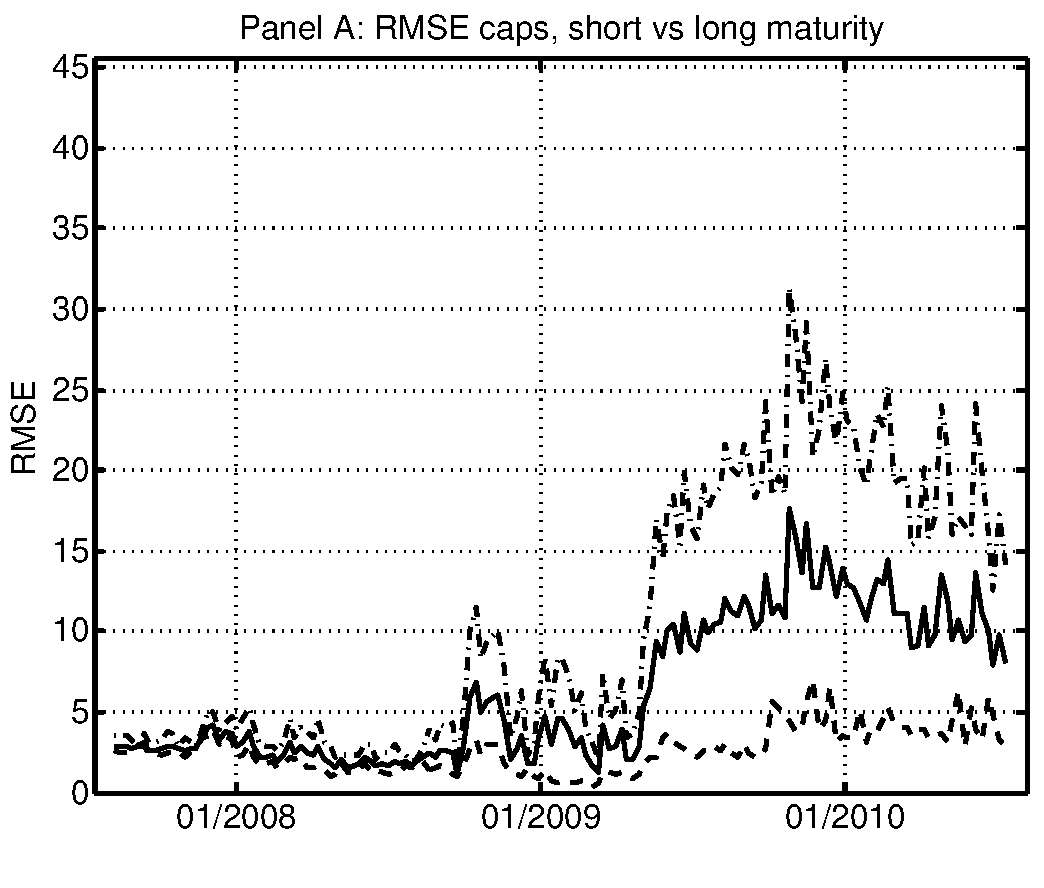
\includegraphics[width=0.5\linewidth]{Graphics/RMSE_ivcapsjoint.pdf} % 'width' argument says max width of this figure must be 0.5* width of  line
\end{figure}

The following subsection presents an example where tables and figures are imported from separate tex files via the \emph{input} command and are referenced to in the text using their labels.

\subsection{Pricing Errors}

[\dots] we present the root mean squared pricing errors (RMSEs) and the mean pricing errors (MPEs) on caps and swaptions implied volatilities, defined as the difference in percentage points between the model-implied values and the market-implied volatility quotes. Overall, we find that, for intermediate and long maturities, our model performs remarkably well. The cap pricing errors in \cref{tbl:Table1} indicate that the model's performance suffers mostly at the short end of option maturities, especially for the one-year maturity. Short maturity contracts are underpriced by the model. However, the pricing performance considerably improves with increasing maturity. For longer maturities, a tendency exists to underprice out-of-the money and overprice in-the-money contracts.

% INPUT TABLE/FIGURE FROM EXTERNAL FILE
\begin{table}[H]
    \caption[Pricing Errors for the Caps Market]{ Pricing errors for the caps market.\label{tbl:Table1}}
    \caption*{Reported are sample averages of the root mean squared errors (RMSEs) and mean pricing
    errors (MPEs) for caps implied volatilities, defined as the difference in percentage points between the model-implied values and the market-implied volatility quotes.
    Each row represents one cap maturity, and columns represent the moneyness of the cap.}
    \setlength{\tabcolsep}{6pt}
    \vspace{0.2cm}
    \begin{tabular}{lcrrrrrrrrrrrr}
    \toprule & \multicolumn{5}{c}{RMSE}
    && \multicolumn{5}{c}{MPE} \\
     \cmidrule(r){2-6}  \cmidrule(r){8-12}
    {Maturity}  & 0.80 & 0.90 & 1.00 & 1.10 & 1.20 && 0.80 & 0.90 & 1.00 & 1.10 & 1.20 \\
    \midrule
    One year  & 16.86   &   18.62   &   20.15   &  20.30   &  22.03 & &  -10.73  & -11.08  & -11.95   &-12.32  &-15.96      \\
    Two years  & 12.26   &   11.71   &    9.79   &   9.57   &   9.85 & &   -8.64  &  -8.77  &  -6.99   & -6.17  & -7.01      \\
    Three years  &  8.78   &    6.75   &    4.75   &   4.19   &   4.02 & &   -6.67  &  -5.15  &  -3.44   & -2.52  & -2.59      \\
    Four years  &  6.47   &    4.29   &    2.25   &   1.66   &   2.03 & &   -4.81  &  -2.98  &  -1.40   & -0.48  & -0.06      \\
    Five years  &  4.98   &    2.94   &    1.35   &   1.26   &   2.18 & &   -3.41  &  -1.67  &  -0.30   &  0.56  &  1.29       \\
    Six years  &  4.28   &    2.36   &    1.41   &   1.68   &   2.50 & &   -2.63  &  -0.92  &   0.31   &  1.11  &  1.97      \\
    Seven years  &  3.91   &    2.16   &    1.71   &   2.08   &   2.71 & &   -2.07  &  -0.38  &   0.74   &  1.48  &  2.25      \\
    Eight years  &  3.63   &    2.07   &    1.89   &   2.27   &   2.80 & &   -1.71  &  -0.07  &   0.95   &  1.63  &  2.33      \\
    Nine years  &  3.48   &    2.09   &    2.04   &   2.42   &   2.88 & &   -1.35  &   0.20  &   1.15   &  1.79  &  2.41      \\
    Ten years &  3.37   &    2.15   &    2.18   &   2.54   &   2.95 & &   -1.06  &   0.42  &   1.31   &  1.91  &  2.47      \\
    \bottomrule
    \end{tabular}\\

\end{table}


For the ATM swaptions implied volatilities in \cref{tbl:Table2}, we observe a similar pattern. The model struggles mostly for short option maturities and short swaption tenors, an observation that also holds true for the non-ATM swaptions. However, across moneyness no clear pattern emerges in terms of over- and underpricing as is the case for in-the-money and out-of-the-money caps.


% INPUT TABLE/FIGURE FROM EXTERNAL FILE
\begin{sidewaystable}
\caption[Pricing Errors for ATM Swaptions]{ Pricing errors for at-the-money (ATM) swaptions.}
\caption*{Reported are sample averages of the root mean squared errors (RMSEs) and mean pricing
errors (MPEs) for ATM swaptions implied volatilities, defined as the difference in percentage points between the model-implied values and the market-implied volatility quotes. Each row represents one swaption maturity, and each column represents one swap tenor.}\label{tbl:Table2}
\vspace{0.2cm}
\setlength{\tabcolsep}{6pt}

\begin{tabular}{lrrrrrrrlrrrrrrr}
\toprule &
\multicolumn{7}{c}{RMSE} &&
\multicolumn{7}{c}{MPE} \\
 \cmidrule(l){2-9}  \cmidrule(l){10-16}
& \multicolumn{7}{c}{Swap tenor} &&
\multicolumn{7}{c}{Swap tenor} \\
 \cmidrule(l){2-9}  \cmidrule(l){10-16}
\multicolumn{1}{l}{{Option}} & \multicolumn{1}{l}{One} & \multicolumn{1}{l}{Two} & \multicolumn{1}{l}{Three} & \multicolumn{1}{l}{Four} &
\multicolumn{1}{l}{Five} & \multicolumn{1}{l}{Seven} & \multicolumn{1}{l}{Ten} & & \multicolumn{1}{l}{One} &  \multicolumn{1}{l}{Two} & \multicolumn{1}{l}{Three} & \multicolumn{1}{l}{Four} & \multicolumn{1}{l}{Five} & \multicolumn{1}{l}{Seven} & \multicolumn{1}{l}{Ten} \\

\multicolumn{1}{l}{maturity} & \multicolumn{1}{l}{year} & \multicolumn{1}{l}{years} & \multicolumn{1}{l}{years} & \multicolumn{1}{l}{years} &
\multicolumn{1}{l}{years} & \multicolumn{1}{l}{years} & \multicolumn{1}{l}{years} & & \multicolumn{1}{l}{year} &  \multicolumn{1}{l}{years} & \multicolumn{1}{l}{years} & \multicolumn{1}{l}{years} & \multicolumn{1}{l}{years} & \multicolumn{1}{l}{years} & \multicolumn{1}{l}{years} \\

\midrule

Three months	&	21.16  & 9.66  &  4.46 & 4.82  & 5.94&8.30  & 10.32 && -14.13  & -7.24&  -1.97&  0.72 &   1.77&  5.09&   7.38\\
Six months	&	19.53  & 7.93  &  2.58 & 2.60  & 3.78&6.17  &  7.89 && -13.67  & -6.05&  -1.45&  0.90 &   1.93&  4.35&   6.10\\
One year	&	12.72  & 5.27  &  1.74 & 1.52  & 2.27&3.82  &  4.95 && -8.81   &-3.21 & -0.43 &  0.86 &  1.48 & 2.83 &  3.84\\
Two years	&	 4.20  & 2.20  &  1.49 & 1.31  & 1.36&1.61  &  2.04 && -1.03   & 0.15 &  0.61 &  0.71 &  0.65 & 0.75 &  1.13\\
Three years	&	 2.34  & 1.75  &  1.38 & 1.18  & 1.13&1.22  &  1.41 &&  1.33   & 1.16 &  0.86 &  0.51 &  0.16 &-0.05 & -0.03\\
Four years	&	 2.36  & 1.65  &  1.29 & 1.08  & 1.19&1.25  &  1.40 &&  1.85   & 1.20 &  0.71 &  0.14 & -0.17 &-0.53 & -0.65\\
Five years	&	 2.36  & 1.65  &  1.35 & 1.25  & 1.32&1.51  &  1.67 &&  1.89   & 1.13 &  0.49 & -0.07 & -0.47 &-0.73 & -0.88\\
Seven years	&	 2.10  & 1.53  &  1.36 & 1.32  & 1.32&1.54  &  1.80	&&  1.44   & 0.73 &  0.28 & -0.16 & -0.44 &-0.74 & -1.07\\
Ten years   &  1.93   & 1.56  &  1.40 & 1.39  & 1.42&1.53  &  1.72 &&  1.32   &0.88  &  0.50 &  0.22 & -0.01 & -0.47& -0.76\\ \bottomrule
\end{tabular}\\
\end{sidewaystable}

The substantially higher pricing errors for the caps and swaptions market at shorter maturities call for further investigation. Ultimately, the caps and swaptions markets must be closely connected, as they both originate from derivatives written on the forward LIBOR. However, during periods of extreme market turmoil, the two markets might exhibit different behaviors due to differences in how the uncertainty regarding the intensified liquidity situation in the interbank market propagates through the caps and swaptions markets. Therefore, we next analyze the behavior of the pricing errors across time to see whether the caps and swaptions market become disintegrated or whether they suffer from the same deficiencies.

In \cref{fig:fig2}, we plot the time series of RMSE (Panel A) and the MPE (Panel B) for caps implied volatilities. We split the time series into long maturities and short maturities. For the first period of our data sample with the financial crisis already in full swing, the pricing errors in terms of RMSE remain remarkably low. In addition, until October 2008, we do not observe a bias in the model's pricing performance with the MPE close to zero. However, the pricing performance deteriorates considerably around April 2009 with substantial underpricing of short maturity contracts. This mispricing remains high until the end of our sample. Interestingly, this period of persistent mispricing of short maturity contracts coincides with the period of high implied volatilities at these maturities. Hence, our model suffers when the volatility term structure is unusually steep.

\begin{figure}[t!]
    \begin{center}
      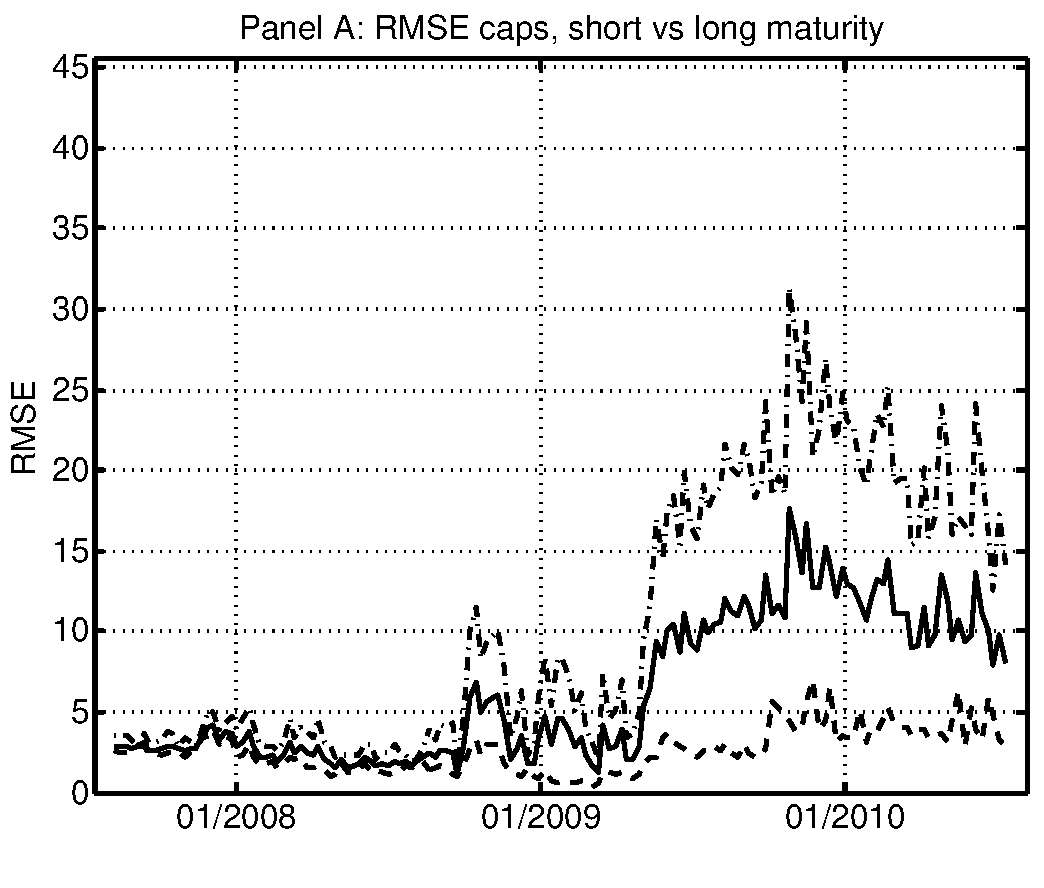
\includegraphics[width=3.20in]{Graphics/RMSE_ivcapsjoint.pdf}
      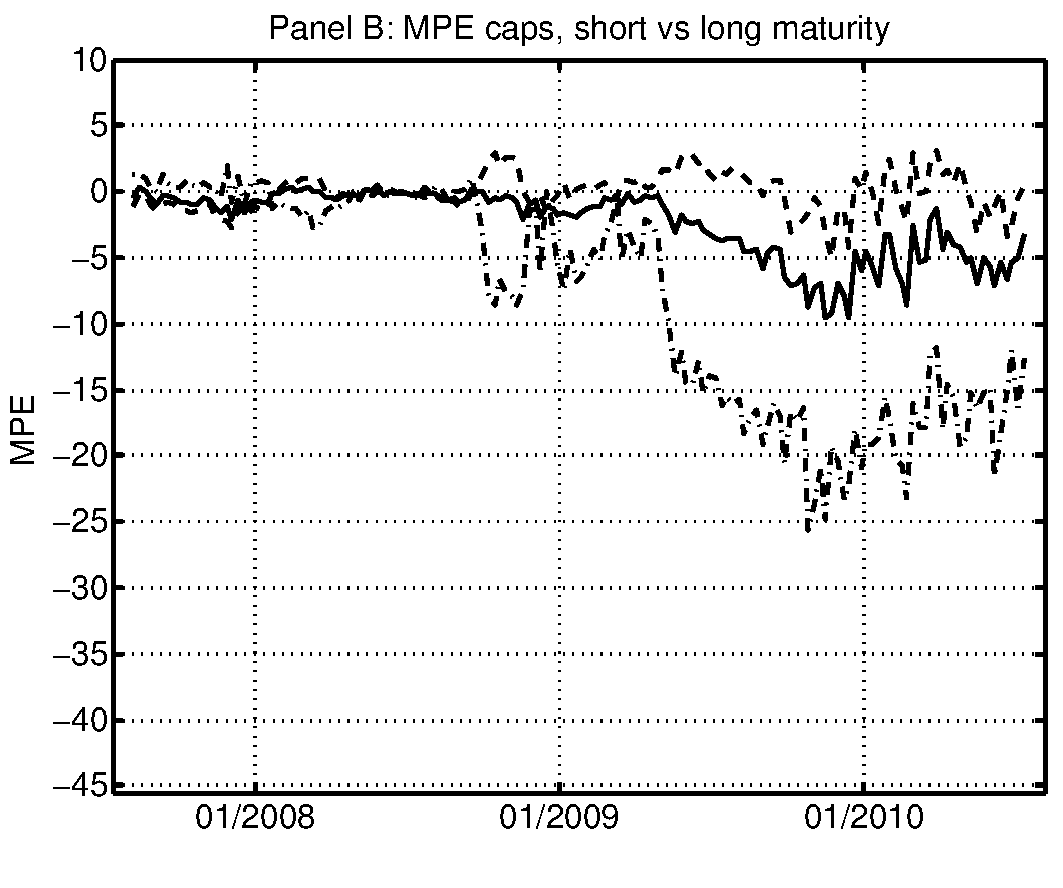
\includegraphics[width=3.20in]{Graphics/MPE_ivcapsjoint.pdf}
    \end{center}
      \caption[RMSE and  MPE for Caps with Different Maturities]{Root mean squared error (RMSE) and mean pricing error MPE for caps with different option maturities.
    Panels A and B show the RMSE and the MPE in percentage points  across time for caps implied volatilities
    of all maturities (solid line), for maturities up to three years (dash-dotted line), and for maturities of four to ten years (dashed line). Data are
    weekly (Wednesday) spanning our entire data sample August 8, 2007 to
    August 11, 2010; in total, 158 weeks.}\label{fig:fig2}
\end{figure}

\subsection{Other environments}
\subsubsection{listings}
The package \emph{listings} is used to present code in your document. But it seems there is a better \href{https://github.com/olivierverdier/python-latex-highlighting}{alternative} for python specific color highlighting.

\begin{lstlisting}[language=Python]
    input numpy as np

    def square_root(x):
        return x**(1/2)
    
    x=4
    assert np.sqrt(x) == square_root(x)
\end{lstlisting}

or Matlab code

\begin{lstlisting}[language=matlab]
figure(1)
set(gca,'Box', 'on', 'LineWidth',1.5 ,'FontSize',14)
plot(x,cumprod(1+R(:,2)),x,cumprod(1+R(:,3)),'--',x,cumprod(1+R(:,4)),'-.','LineWidth',1.5)
grid on
datetick('x','mmmyy')
axis([x(1)-10 x(end) 0.5 3.0])
title('Panel A: Equity and commodity indices')
ylabel('Cumulative return')
grid on
legend('MSCI World Total Return', 'MSCI Emerging Market Total Return','DJ UBS Commodity Index')
print('-depsc2', 'cumReturnA.eps' )
\end{lstlisting}



\subsection{A Note on Referencing}
\subsubsection{Bibliography}
There are basically two options to include citations and references to your document: Bibtex or BibLatex. This doc is constructed using the latter, because it's newer and more flexible (e.g.\ allows use in \emph{beamer} documentclass). There are different citing commands, each with a slightly different outcome:~\cite{BA1996}, \textcite{CW2004} and \parencite{SH1993,BA1996}. You can also combine citations, \textcite{petkova2006fama,CW2004}. \emph{textcite} is the one most commonly used, though \emph{parencite} is useful too.

\subsubsection{Other\label{sec:this_section}}
There is also the option to refer to many other things (floats, footnotes, (sub)sections,\ldots).  With the \emph{cleverref} package, you can easily refer to these object by using the `cref' command.  \cref{eq:CAPM}, \cref{fig:a_fig}, \cref{ft:randomfootnote}, \cref{sec:this_section}, \cref{tbl:try_table}. You can also combine references of the same type of objects, just like citations, \cref{eq:CAPM,eq:FF3}.

[Here are some examples of citations\dots] Lévy processes cannot capture stochastic volatility, stochastic risk reversal (skewness) and stochastic correlation. These drawbacks can be resolved, at least to some extent, by considering time-changed Lévy processes for which it is possible to generate distributions which vary over time. If the return innovation is modeled by a Brownian motion, we can let the instantaneous variance be stochastic (see, e.g., \textcite{SH1993,BA1996}) to create dependence of the return increments.\footnote{\textcite{CW2004}, for instance, introduced a time-changed Lévy model to capture the leverage effect.} 


%--------------------
% CHAPTER 2
%--------------------

\chapter{ [ Chapter Title ]}

\section{ [ Section Title ] }

\subsection{ [  Subsection Title ] }

%----------------------------------------------------------------------------------------
% APPENDIX
%----------------------------------------------------------------------------------------

\appendix
\begingroup
\makeatletter
\let\ps@plain\ps@empty
\appendixpage
\makeatother
\endgroup
\noappendicestocpagenum
\addappheadtotoc


\renewcommand{\theequation}{A.\arabic{equation}}

\chapter{Proofs\label{chp:proofs}}

[ You may also want to add an appendix, if it makes sense. You delegate proofs to the appendix or other material that is essential for the understanding of your work, but would distract the reader if placed in the main text\dots ]

\section{Proof of Proposition [\dots]\label{sec:proof_prop1}}
[\dots.], we can apply Ito's formula for Lévy processes   to obtain the
dynamics of the forward LIBOR \(L(t,T_j)\) to obtain the
dynamics of the forward LIBOR \(L(t,T_j)\) under the \(T_{j+1}\)-forward measure
as follows:
\begin{eqnarray}
\frac{dL(t,T_j)}{L(t,T_j)} &=& b (t,T_{j},T_{j+1}) dt +
\frac{1}{2} \lambda ^2(t,T_j) dt +
\frac{1}{2} V _t^W dt\nonumber \\
&+& \int_{-\infty}^{0}  \left[ e^{x}-1-x \right]
\pi_{J^-}^{\mathbb Q_{j+1}}(dx)\nu _t^J dt + \int_{0}^{\infty} \left[
e^{x}-1-x \right] \pi_{J^+}^{\mathbb Q_{j+1}}(dx)\nu _t^J dt \nonumber \\
&+& \lambda (t,T_j) dB_{t}^{Q_{j+1}}+ \sqrt{ V _t^W}
dW_{t}^{Q_{j+1}}+ \int_{-\infty}^{0} \left[ e^{ x}-1 \right]
\left[ \mu^- (dt,dx) -
\pi_{J^-}^{Q_{j+1}}(x) dx \nu _t^J dt \right]\nonumber \\
&+& \int_{0}^{\infty} \left[ e^{ x}-1 \right] \left[ \mu ^+ (dt,dx)
- \pi_{J^+}^{Q_{j+1}}(x) dx \nu _t^J dt \right].\label{eq:app_eq}
\end{eqnarray}
To ensure that \(L(t,T_j)\) is a martingale under the
\(T_{j+1}\)-forward measure, the drift must equal zero, which gives the
drift condition in the proposition. \(\blacksquare\)

%----------------------------------------------------------------------------------------
% BIBLIOGRAPHY
%----------------------------------------------------------------------------------------
\printbibliography\

\newpage


%----------------------------------------------------------------------------------------
%
%----------------------------------------------------------------------------------------
\thispagestyle{firststyle}

\section*{Eidesstattliche Erklärung}
Der/Die Verfasser/in erklärt an Eides statt, dass er/sie die vorliegende Arbeit selbständig, ohne fremde Hilfe und ohne Benutzung anderer als die angegebenen Hilfsmittel angefertigt hat. Die aus fremden Quellen (einschliesslich elektronischer Quellen) direkt oder indirekt übernommenen Gedanken sind ausnahmslos als solche kenntlich gemacht. Die Arbeit ist in gleicher oder ähnlicher Form oder auszugsweise im Rahmen einer anderen Prüfung noch nicht vorgelegt worden.\\[2cm]
\dotbox{Ort, Datum} \hfill \dotbox{Unterschrift des/der Verfassers/in}


\end{document}
